\documentclass[border=5pt, multi, tikz]{standalone}
\usepackage{tikz}
\usepackage{amsfonts,amssymb,amsmath}
\usepackage{xcolor}
\begin{document}
\newcommand{\Depth}{1.5}
\newcommand{\Height}{2}
\newcommand{\Width}{2.2}



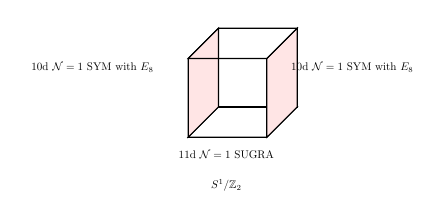
\begin{tikzpicture}
\coordinate (O) at (0,0,0);
\coordinate (A) at (0,\Width,0);
\coordinate (B) at (0,\Width,\Height);
\coordinate (C) at (0,0,\Height);
\coordinate (D) at (\Depth,0,0);
\coordinate (E) at (\Depth,\Width,0);
\coordinate (F) at (\Depth,\Width,\Height);
\coordinate (G) at (\Depth,0,\Height);

\draw[black] (O) -- (C) -- (G) -- (D) -- cycle;% Bottom Face
\draw[black] (O) -- (A) -- (E) -- (D) -- cycle;% Back Face
\draw[black,fill=red!10] (O) -- (A) -- (B) -- (C) -- cycle;% Left Face
\draw[black,fill=red!10] (D) -- (E) -- (F) -- (G) -- cycle;% Right Face
\draw[black] (C) -- (B) -- (F) -- (G) -- cycle;% Front Face
\draw[black] (A) -- (B) -- (F) -- (E) -- cycle;% Top Face


  \node at (-1.6,.5) [scale=0.4] {10d $\mathcal{N}=1$ SYM with $E_8$};
  \node at (1.7,.5) [scale=0.4] {10d $\mathcal{N}=1$ SYM with $E_8$};
  \node at (0.1,-.6) [scale=0.4] {11d $\mathcal{N}=1$ SUGRA};
  \node at (0.1,-1) [scale=0.4] {$S^1/\mathbb{Z}_2$};

%% Following is for debugging purposes so you can see where the points are
%% These are last so that they show up on top
%\foreach \xy in {O, A, B, C, D, E, F, G}{
%    \node at (\xy) {\xy};
%}
\end{tikzpicture}
\end{document}


\begin{document}
\begin{tikzpicture}
  \pic at (1,-3) {annotated cuboid={width=150, height=200, depth=250, scale=.01, units=m}};
  \node at (0,-2) [scale=0.5] {$\mathcal{N}=1$ with $E_8$};
\end{tikzpicture}
\end{document}